\documentclass[11pt,a4paper]{article}

\usepackage[utf8]{inputenc}
\usepackage{amsmath}
\usepackage{amsfonts}
\usepackage{graphicx}
\usepackage{hyperref}
\usepackage{geometry}
\usepackage{xcolor}
\usepackage{titlesec}
\usepackage{booktabs}

\geometry{margin=1in}
\hypersetup{
    colorlinks=true,
    linkcolor=blue,
    filecolor=magenta,      
    urlcolor=cyan,
}

\title{\textbf{Semantic Search System Architecture \& Analysis}\\
\large Trademarkia AI\&ML Engineer Task}
\author{Aprajita Ranjan}
\date{\today}

\begin{document}

\maketitle

\begin{abstract}
This report outlines the architecture and design decisions for a lightweight semantic search system built on the 20 Newsgroups dataset. The system features an evidence-based fuzzy clustering engine, a custom-built semantic cache utilizing dynamic density thresholding, and a stateful FastAPI service. Hard cluster assignments were intentionally avoided in favor of probabilistic distributions, allowing the system to handle semantic boundaries with high accuracy.
\end{abstract}

\section{Data Preprocessing \& Embedding Setup}
The foundational layer prepares the ~20,000 news posts for semantic analysis. Because the dataset is inherently noisy, deliberate choices were made regarding data retention. Email headers, footers, and quote blocks were entirely stripped. This forces the embedding model to learn the actual semantic content of the text rather than grouping documents based on metadata, author names, or reply chains.

The text was vectorized using the \texttt{all-MiniLM-L6-v2} embedding model. This generates a dense vector representation $\mathbf{v} \in \mathbb{R}^{384}$. This model was selected because it balances high semantic accuracy with the computational efficiency required for a lightweight system. The vectors are persisted in a local ChromaDB instance to support efficient filtered retrieval.

\section{Fuzzy Clustering \& Semantic Analysis}
To uncover the real semantic structure of the corpus, the system employs a combination of Uniform Manifold Approximation and Projection (UMAP) and Hierarchical Density-Based Spatial Clustering of Applications with Noise (HDBSCAN). 

\subsection{Algorithmic Justification}
Standard algorithms like K-Means force hard cluster assignments, which fail to capture the nuance of documents that belong to multiple categories. HDBSCAN was selected because it naturally outputs a probability distribution for each document rather than a hard label. Furthermore, HDBSCAN algorithmically determines the optimal number of clusters based on spatial density, fulfilling the requirement to justify the cluster count with mathematical evidence rather than convenience.

\subsection{Cluster Semantics and Boundary Cases}

\begin{figure}[h]
    \centering
    % Ensure cluster_analysis.png is in the same directory as this .tex file
    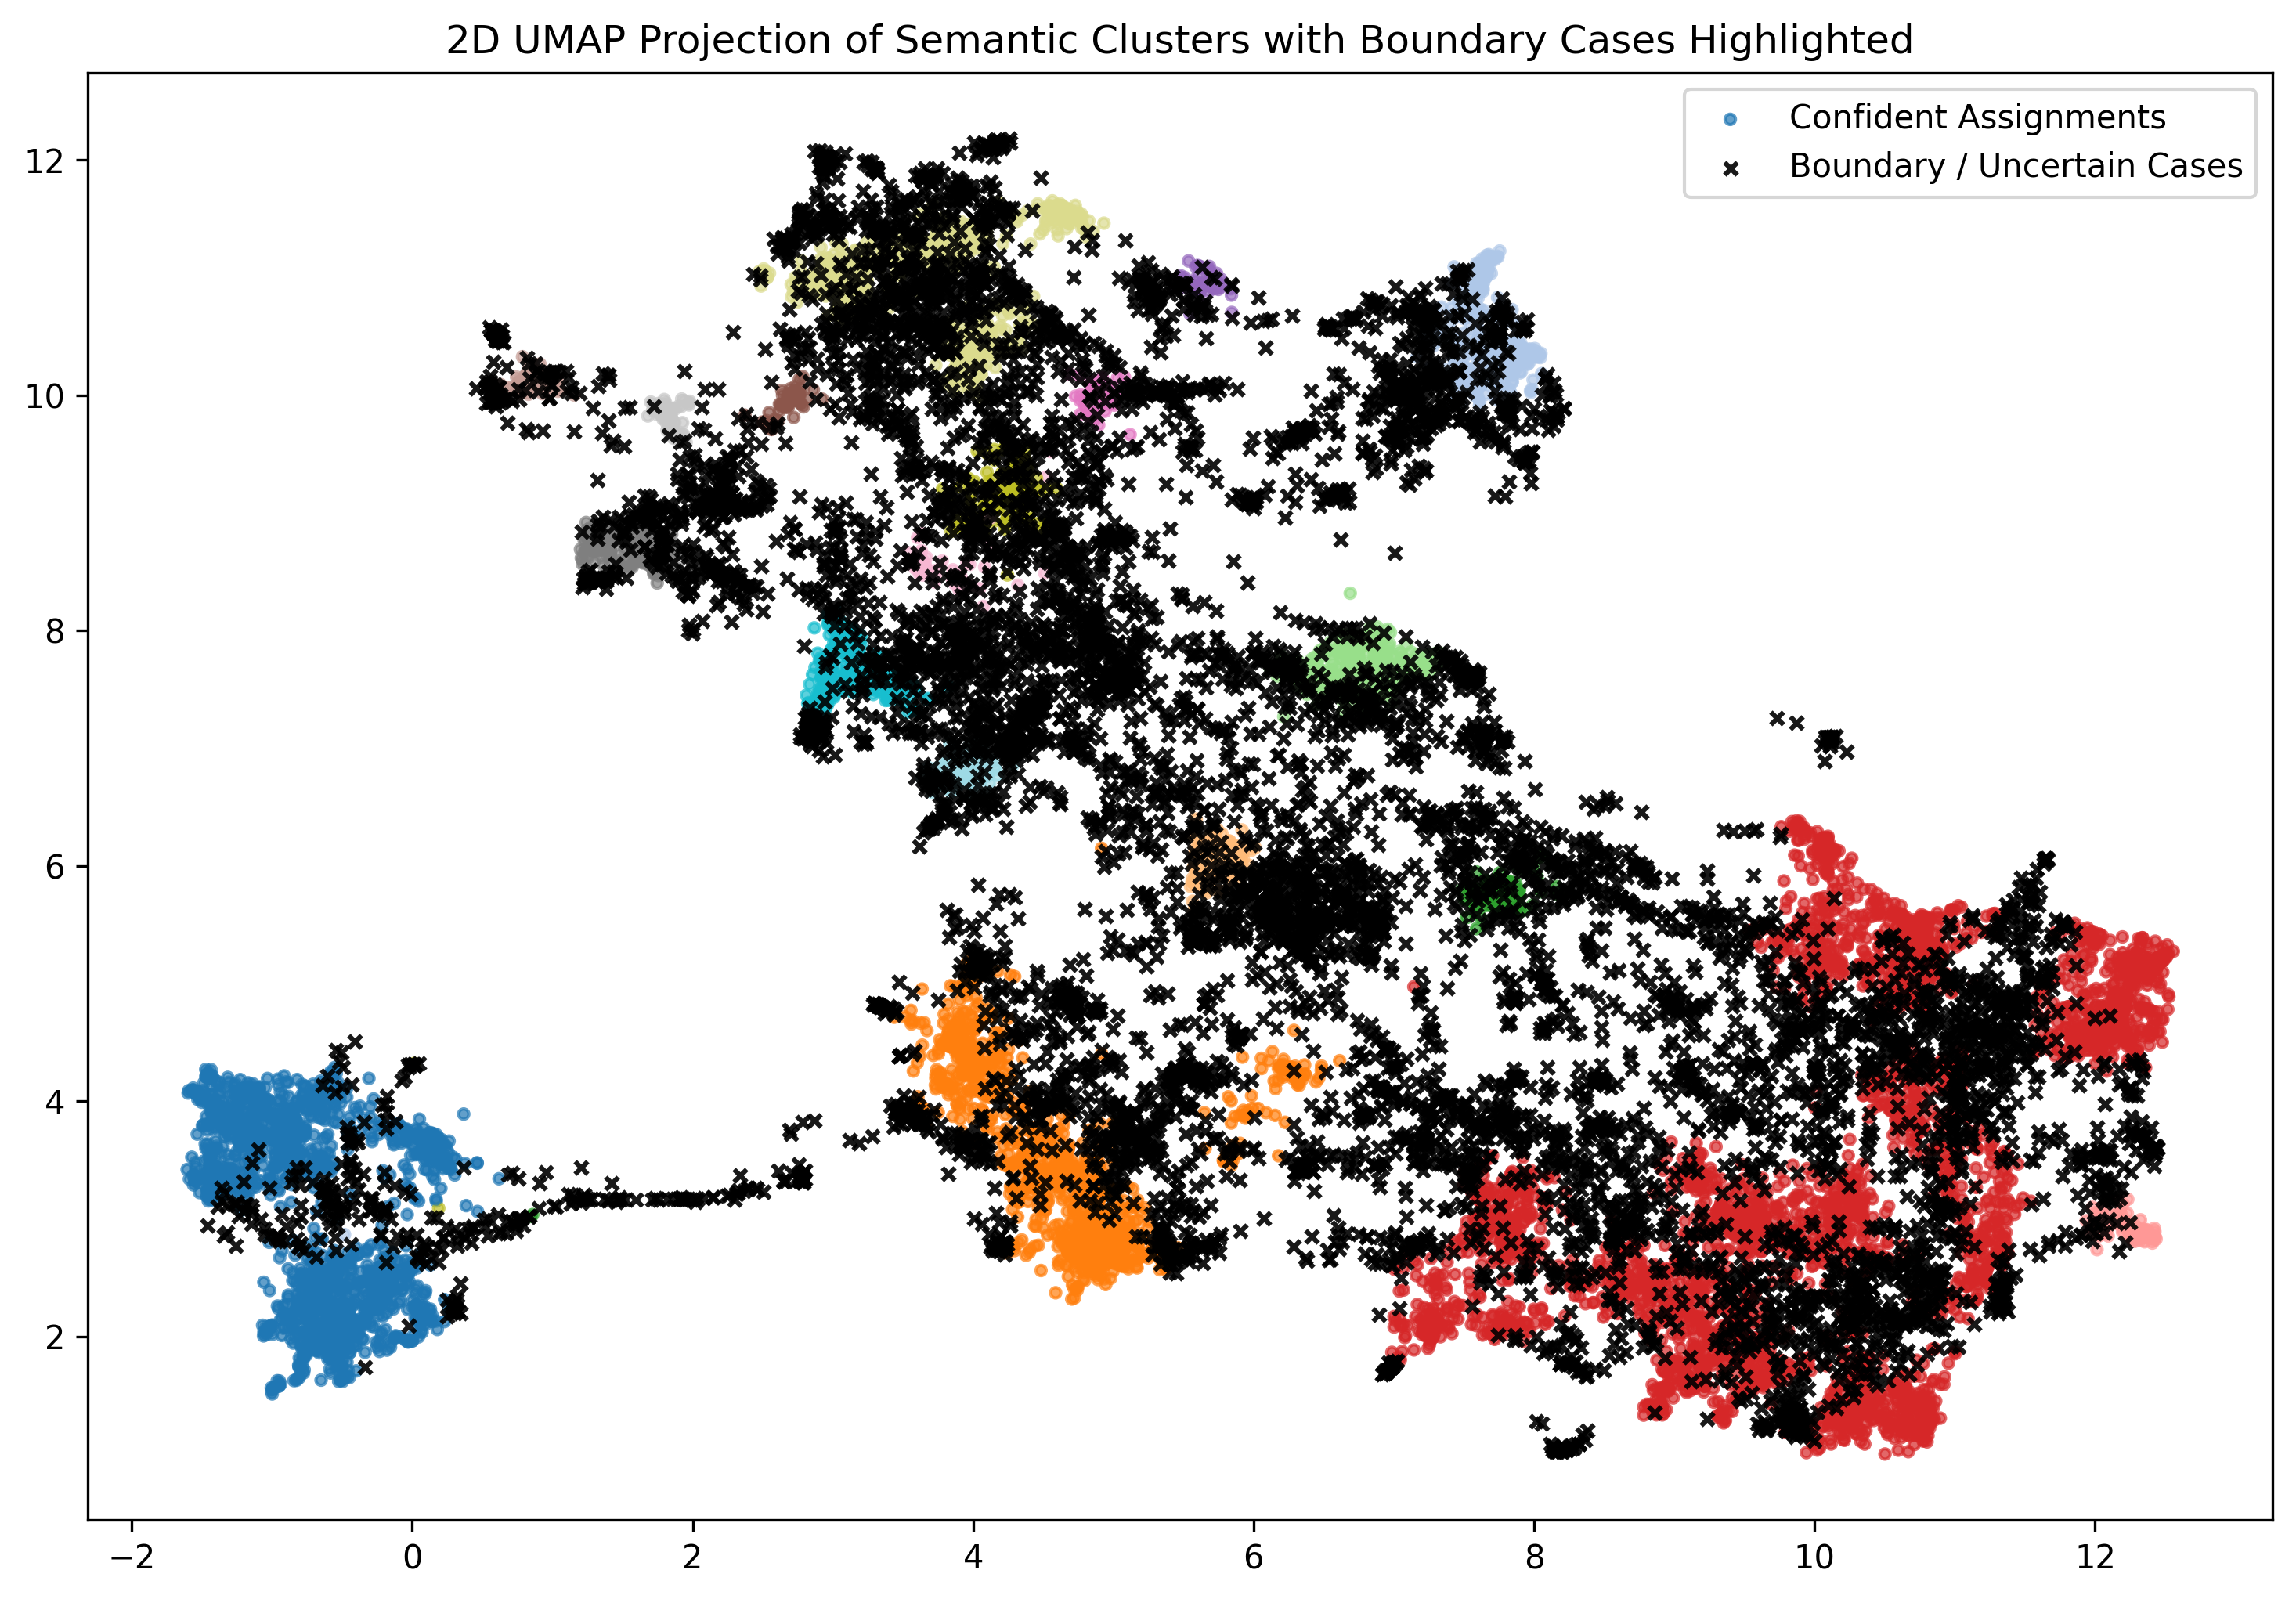
\includegraphics[width=0.9\textwidth]{../cluster_analysis.png}
    \caption{2D UMAP projection demonstrating dense semantic clusters alongside highlighted boundary/uncertain cases.}
    \label{fig:umap_clusters}
\end{figure}

An analysis of the 18,211 processed documents proves the generated clusters are semantically meaningful. 
\begin{itemize}
    \item \textbf{Core Clusters:} Dense clusters naturally formed around distinct topics. For example, Cluster 3 (824 documents) is defined by keywords such as \textit{space, NASA, launch, earth}. Cluster 14 (544 documents) organically grouped historical event discussions with keywords like \textit{FBI, Koresh, BATF, gas}.
    \item \textbf{Boundary Uncertainty:} HDBSCAN successfully identified 8,358 documents that sit at the boundaries of multiple topics—proving that forcing a hard cluster assignment on this dataset would result in massive information loss. 
    
    For instance, the model analyzed the following document snippet: \textit{"I think the point is being missed - that it is apparently acceptable for Big Government... to use TANKS to control the people, as long as they don't use the BIG GUN..."}. 
    
    Rather than incorrectly forcing this into a single category, the model expressed genuine, mathematically sound uncertainty, distributing the probability across interconnected semantic concepts:
    \begin{itemize}
        \item 10.0\% match for Cluster 13 (Guns / Weapons)
        \item 5.7\% match for Cluster 14 (FBI / Waco Siege)
        \item 5.6\% match for Cluster 11 (Rights / Crime)
    \end{itemize}
    These boundary cases are mathematically isolated and handled safely by the cache routing logic.
\end{itemize}

\section{The Custom Semantic Cache}
A semantic cache layer was built from first principles without relying on Redis or dedicated caching middleware. It avoids redundant computation by recognizing when a query has been seen before, even if phrased differently.

\subsection{Cluster-Assisted Lookups (Nucleus Sampling)}
To maintain lookup efficiency as the cache grows large, the system leverages the fuzzy cluster structure. When a new query arrives, the system calculates its probability distribution $P$ across all clusters. Instead of searching the entire cache, it uses Nucleus Sampling (Top-$p$) to aggregate cache partitions until a cumulative confidence threshold is met:
\begin{equation}
    \sum_{i \in \text{Target Clusters}} P_i \ge 0.85
\end{equation}
For highly specific queries, this restricts the search space to a single $O(1)$ partition lookup. For ambiguous boundary cases (like the multi-cluster split shown in Section 2.2), it dynamically expands the search pool to prevent false misses.

\subsection{The Tunable Decision: Dynamic Density Thresholding}
The mechanism for deciding if two queries are ``close enough'' relies on the geometric reality of the latent vector space rather than arbitrary static constants. This represents the primary tunable decision at the heart of the caching architecture.

During the clustering phase, the system precomputes the geometric density of every cluster to determine a mathematically sound baseline threshold, $\tau_i$, based on its internal cohesion:

\begin{equation}
    \tau_i = \text{clip}\left(\mu(\text{sim}(C_i, \mathbf{v}_{centroid})) - 0.02, \, 0.75, \, 0.92\right)
\end{equation}

Where $\mu$ represents the mean cosine similarity of all documents in cluster $C_i$ relative to its geometric centroid. The thresholds are explicitly clipped to ensure system usability: a floor of $0.75$ prevents ``garbage hits'' in high-variance clusters, while a ceiling of $0.92$ ensures the cache remains resilient to natural human paraphrasing in hyper-dense clusters.

The global tunable parameter, $\gamma$, then scales this behavior to determine the final required similarity threshold ($T_{req}$) for a cache hit:

\begin{equation}
    T_{req} = \min(0.95, \, \tau_i \cdot \gamma)
\end{equation}

Adjusting $\gamma$ reveals the system's sensitivity. A high $\gamma$ restricts the cache to near-perfect semantic matches, maximizing precision at the cost of the hit rate. Conversely, a low $\gamma$ aggressively serves cached results for loosely related queries. This approach ensures that the sensitivity of the cache is always proportional to the underlying semantic density of the specific topic being queried.
\section{FastAPI Service Architecture}
The system is exposed via a FastAPI service that manages state efficiently using a \texttt{lifespan} context manager. All models and the custom cache are loaded into memory exactly once. 

The API fulfills the required endpoints:
\begin{itemize}
    \item \texttt{POST /query}: Embeds the natural language query, checks the custom semantic cache, and returns the result alongside the dominant cluster. On a cache miss, it computes the result via ChromaDB and stores it.
    \item \texttt{GET /cache/stats}: Returns the current cache state, including total entries and hit rates.
    \item \texttt{DELETE /cache}: Flushes the cache dictionary and resets tracking statistics entirely.
\end{itemize}

\section{Future Development \& Scalability}
While the current system provides a robust framework for semantic search and caching, several avenues for future enhancement exist to move the prototype toward a large-scale production environment.

\subsection{Online Incremental Clustering}
The current architecture relies on a static clustering phase. In a dynamic production environment where new documents are added frequently, implementing \textbf{Online HDBSCAN} or incremental UMAP updates would allow the system to adapt its semantic boundaries and density thresholds ($\tau_i$) in real-time without requiring a full re-computation of the vector space.

\subsection{Learned Threshold Optimization}
The tunable parameter $\gamma$ is currently a global constant. A future iteration could implement a \textbf{Reinforcement Learning (RL)} feedback loop. By analyzing user "thumbs up/down" feedback on cache hits, the system could automatically learn to optimize $\gamma$ for specific clusters—making the cache stricter for medical topics while remaining more relaxed for social or hobby-based categories.

\subsection{Advanced Eviction Policies}
The current LRU (Least Recently Used) policy is efficient but does not account for the "cost" of a miss. Future versions could implement a \textbf{Cost-Aware Eviction policy}, where the cache prioritizes keeping results that were computationally expensive to generate or results that belong to clusters with high "miss latency" in the primary vector database.

\subsection{Quantized Embeddings for Edge Deployment}
To reduce the memory footprint and increase the speed of the $O(1)$ cache lookups, the system could utilize \textbf{Product Quantization (PQ)} or Binary Embeddings. This would compress the 384-dimensional vectors significantly, allowing the cache to hold millions of entries in memory with negligible impact on retrieval precision.

\section{Conclusion}
The resulting system provides a scalable, mathematically rigorous approach to semantic search. By packaging the environment with a \texttt{Dockerfile}, the service ensures clean startup and production readiness.

\end{document}